%%%%%%%%%%%%%%%%%%%%%%%%%%%%%%%%%%%%%%%%%%%%%%%%%%%%%%%%%%%%%%%%%%%%%%%%%
% ARTICLE ABOUT FATE OF SYNONYMOUS MUTATIONS IN HIV
%%%%%%%%%%%%%%%%%%%%%%%%%%%%%%%%%%%%%%%%%%%%%%%%%%%%%%%%%%%%%%%%%%%%%%%%%
\documentclass[12pt,a4paper,notitlepage,onecolumn]{article}
%%%%%%%%%%%%%%%%%%%%%%%%%%%%%%%%%%%%%%%%%%%%%%%%%%%%%%%%%%%%%%%%%%%%%%%%%
\newcommand{\Author}{Fabio~Zanini and Richard~A.~Neher}
\newcommand{\Title}{(Rise and fall of synonymous mutations)}
\newcommand{\Keywords}{{HIV}, {synonymous}, {population genetics}}
%%%%%%%%%%%%%%%%%%%%%%%%%%%%%%%%%%%%%%%%%%%%%%%%%%%%%%%%%%%%%%%%%%%%%%%%%
\usepackage[english]{babel}
\usepackage[utf8x]{inputenc}
\usepackage{amsmath,amsfonts,amssymb,eucal,eurosym}
\usepackage{color}
\usepackage{subfig}
\usepackage{graphicx}
%\usepackage[font=small, format=hang, labelfont={sf,bf}, figurename=Fig.]{caption}
\usepackage{natbib}
\usepackage{pslatex}
\usepackage[colorlinks,linkcolor=red,citecolor=red]{hyperref}
\hypersetup{pdfauthor={\Author}, pdftitle={\Title}, pdfkeywords={\Keywords}}
%%%%%%%%%%%%%%%%%%%%%%%%%%%%%%%%%%%%%%%%%%%%%%%%%%%%%%%%%%%%%%%%%%%%%%%%%
\graphicspath{{./figures/}}
%%%%%%%%%%%%%%%%%%%%%%%%%%%%%%%%%%%%%%%%%%%%%%%%%%%%%%%%%%%%%%%%%%%%%%%%%
%\DeclareMathOperator\de{d\!}
\newcommand{\comment}[1]{\textit{\textcolor{red}{#1}}}
\newcommand{\mut}{\mu}
\newcommand{\mfit}{\langle F\rangle}
\newcommand{\mexpfit}{\langle e^{F}\rangle}
\newcommand{\ox}{r}
\newcommand{\co}{\rho}
\newcommand{\gt}{g}
\newcommand{\locus}{s}
\newcommand{\locuspm}{t}
\newcommand{\OO}{\mathcal{O}}
\newcommand{\env}{\textit{env}}
\newcommand{\rev}{\textit{rev}}
%%%%%%%%%%%%%%%%%%%%%%%%%%%%%%%%%%%%%%%%%%%%%%%%%%%%%%%%%%%%%%%%%%%%%%%%%
\title{\Title}
\author{\Author}
\date{\today}
%%%%%%%%%%%%%%%%%%%%%%%%%%%%%%%%%%%%%%%%%%%%%%%%%%%%%%%%%%%%%%%%%%%%%%%%%
\begin{document}
%%%%%%%%%%%%%%%%%%%%%%%%%%%%%%%%%%%%%%%%%%%%%%%%%%%%%%%%%%%%%%%%%%%%%%%%%
\maketitle

\begin{abstract}
\noindent
Intrapatient HIV evolution is goverened by selection on the protein level in the
arms race with the immune system (killer T-cells and antibodies). Synonymous
mutations do not have an immunity-related phenotype and are often assumed to be
neutral. In this paper, we show that synonymous changes in epitope-rich regions
are often deleterious but still reach frequencies of order one.  We analyze time
series of viral sequences from the V1-C5 part of {\it env} within individual
hosts and observe that synonymous derived alleles rarely fix in the
viral population. Simulations suggest that such synonymous mutations
have a (Malthisuan) selection coefficient of the order of $-0.001$, and that
they are brought up to high frequency by linkage to neighbouring beneficial
nonsynonymous alleles (genetic draft). As far as the biological causes are
concerned, we detect a negative correlation between fixation of an allele and
its involvement in evolutionarily conserved RNA stem-loop structures.
This phenonenon is not observed in other parts of the HIV genome, in which
selective sweeps are less dense and the genetic architecture less constrained.
%In absence of antiretroviral treatment, HIV is very successful at producing
%mutants that are able to stay undetected by the host immune system for months,
%boosting the infection~\citep{richman_rapid_2003, bunnik_autologous_2008,
%moore_limited_2009}. The high mutation rate at the core of this process,
%however, also generates genetic noise in the background of beneficial alleles.
%Because of the limited ourcrossing of HIV, hitchhikers usually stay linked to
%the focal allele for a time comparable to its sweeping time, i.e. a few
%months~\citep{neher_recombination_2010, batorsky_estimate_2011}. The later fate
%of these accessory mutations depends more and more, as they decouple genetically
%from the escape allele via recombination, on their own fitness effects. In this
%study we show that, in a genetic region particularly dense of selective sweeps,
%synonymous hitchhikers tend to revert on a time scale of the order of 500 days,
%because of their deleterious fitness effects. In addition, we provide evidence
%that the biological origin for this deleterious effects resides, at least
%partially, in the disruption of macroevolutionarily conserved RNA secondary
%structures, termed ``insulating stems''.
\end{abstract}

\section{Introduction}

HIV evolves rapidly within a single host during the course of the infection. The
driving forces shaping this process are the high mutation rate and the strong
selection imposed by the host immune system via killer T cells (CTLs) and
neutralizing antibodies (AB)~\citep{pantaleo_immunopathogenesis_1996}.

When the host develops a CTL or AB respose against a particular viral epitope,
rare HIV variants carrying mutated versions of the epitope, called {\it escape
mutants}, acquire a fitness advantage and spread rapidly in the viral
population, within a few months (see \figurename~\ref{fig:aft}, solid lines).
During chronic infection, the (Malthusian) effect size of this beneficial
mutations is of the order of $s_e \sim 0.01$~\citep{neher_recombination_2010}.
The viral \env{} gene shows the fastest rates of adaptation, because is both
rich of CTL epitopes and targeted by antibodies; its sequence diverges at rates
of the order of $1\%$ per year~\citep{shankarappa_consistent_1999}.

Many nucleotide polymorphisms that reach high frequency in the viral population
are escape mutations: all of them are {\it nonsynonymous} (i.e. they appear in
protein coding regions and change the amino acid sequence). Nonetheless,
nucleotide changes unrelated to immune escape are not rare, in \env{} and
elsewhere, and some of them become abundant alike, often rapidly. In particular,
it is not uncommon for {\it synonymous} mutations to reach frequencies of order
one within months from their first appearance (see \figurename~\ref{fig:aft},
dashed lines). The biological function of these mutations within the economy of
HIV is not well understood. By definition, the immunological phenotype, which is
decided at the protein level, is unaffected, but other biological and ecological
aspects of the viral lifestyle might be involved. In practice, a couple of
RNA-level phenotypes are known. For example, within \env{} a certain RNA
sequence, called \rev{} response element (RRE), is used by HIV to enhance
nuclear export of some of its transcripts~\citep{fernandes_hiv-1_2012}. Another
well studied case is the interaction between viral reverse transcriptase, viral
ssRNA, and the host tRNA$^\text{Lys3}$: the latter is required for priming
reverse transcription (RT) and bound by a specifical pseudoknotted RNA structure
in the viral 5' untranslated region~\citep{barat_interaction_1991,
paillart_vitro_2002}.

Crucially for evolutionary purposes, the minor phenotypes caused by synonymous
mutations might have an effect on viral fitness. For instance, recent studies
have shown that genetically engineered HIV strains with skewed codon usage bias
(CUB) patterns towards more or less abundant tRNAs replicate better or worse,
respectively~\citep{ngumbela_quantitative_2008, li_codon-usage-based_2012}. In
this study, we try to characterize the fitness effects of synonymous
polymorphisms that, at some point during chronic infection, become abundant in
the viral population.

One simple way to assess the neutrality of synonymous mutations is to look at
their level of conservation. Deleterious mutations at functional sites are
expected to be absent or rare across the viral population; vice versa, mutant
alleles that reach high frequencies are expected to be neutral. If genetic sites
are independent, the equilibrium frequency of a deleterious allele with fitness
$-s$ is $\mut / |s|$, where $\mut$ is the mutation rate per site per generation;
neutral alleles have no equilibrium frequency and can slowly fix via genetic
drift~\citep{ewens_mathematical_2004}. If the focal synonymous mutant is linked
to another nonneutral allele, however, its frequency is the result of the
combined fitness effects of both sites, and simple conservation-level analyses
fail. Since recombination in HIV is known to happen
rarely~\citep{neher_recombination_2010, batorsky_estimate_2011}, the genetic
context of the synonymous change at hand must be taken into account. Our
results underline the importance of the latter scenario for intrapatient HIV
evolution.

\section{Results}
We analyze from time series of viral nucleotide sequences from single patients,
which span several years of chronic
infection~\citep{shankarappa_consistent_1999, bunnik_autologous_2008,
liu_selection_2006}. Plotting the allele frequencies against time for all
polymorphic sites, it is evident that, although nonsynonymous changes are
widespread, synonymous ones are also present in various occasions at high
frequency (see \figurename~\ref{fig:aft}).
\begin{figure}
\begin{center}
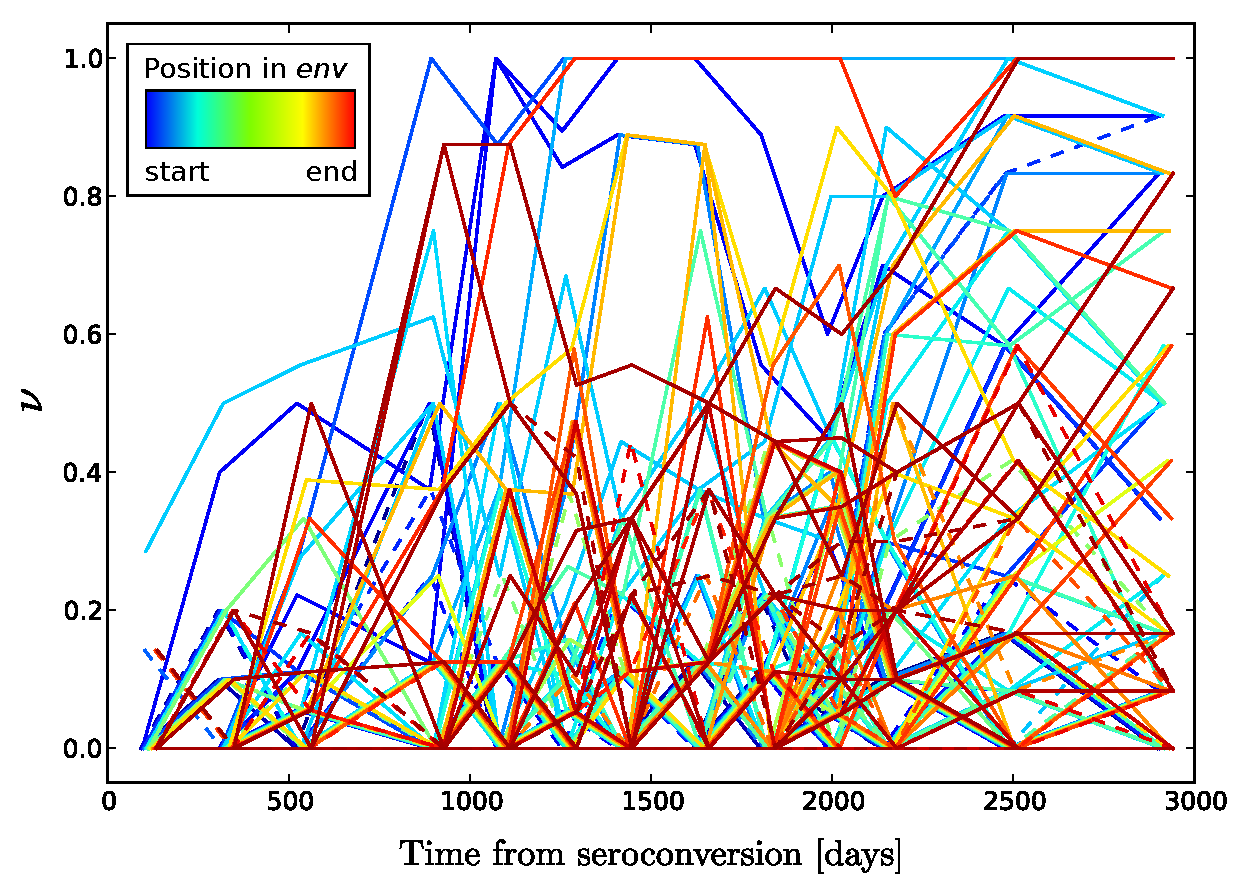
\includegraphics[width=\linewidth]{Shankarappa_allele_freqs_trajectories_syn_nonsynp8}
\caption{Allele frequency trajectories of typical patient, C3-V5, nonsynonymous
(solid) and synonymous mutations (dashed lines). Most synonymous mutations are
not fixed. Colors are set according to the position of the site along the C3-V5
region (red to blue). Data from Ref.~\cite{shankarappa_consistent_1999}.}
\label{fig:aft}
\end{center}
\end{figure}
Moreover, many mutations appear to change rapidly in frequency as a flock,
especially at the lower end of the frequency spectrum. These observations lead
to the idea that linkage might be widespread at the time scale of the typical
selective sweep, i.e. a few months~\citep{neher_recombination_2010}. It seems
therefore likely that synonymous mutations are not attaining high frequencies by
genetic drift but are rather exponentially amplified by selection on linked
nonsynonymous sites, a process known as {\it genetic
draft}~\citep{neher_genetic_2011}.

To test this hypothesis, we focus on the long-time fate of such synonymous
derived alleles {\it after} they are already abundant. According to the neutral
theory of independent sites, (a) an allele starting at frequency $\nu$ will
reach fixation, in the long-time limit, with a probability $P_f(\nu) = \nu$, and
get extinct otherwise; (b) the time required to reach either boundary, fixation
or extinction, is essentialy the inverse of the population size (in
generations), hence much longer than five years for HIV~\citep{boltz_ultrasensitive_2012}.
\begin{figure}
\begin{center}
\subfloat{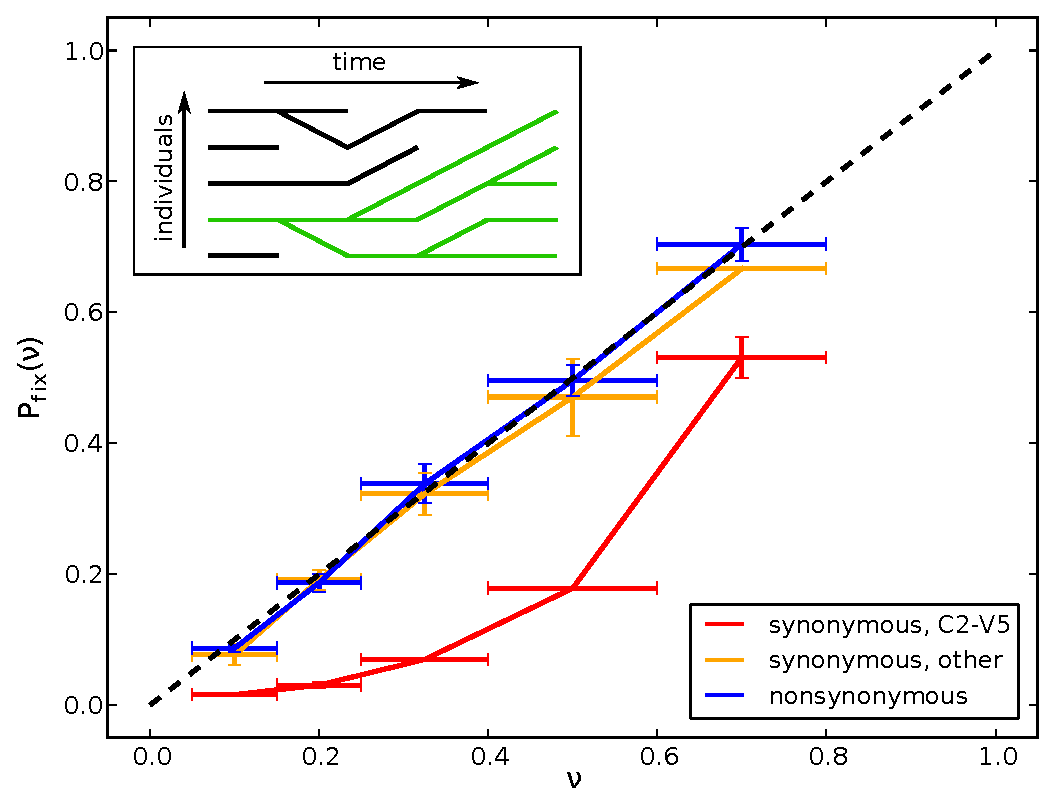
\includegraphics[width=0.49\linewidth]{Bunnik2008_fixmid_syn_ShankanonShanka}}
\subfloat{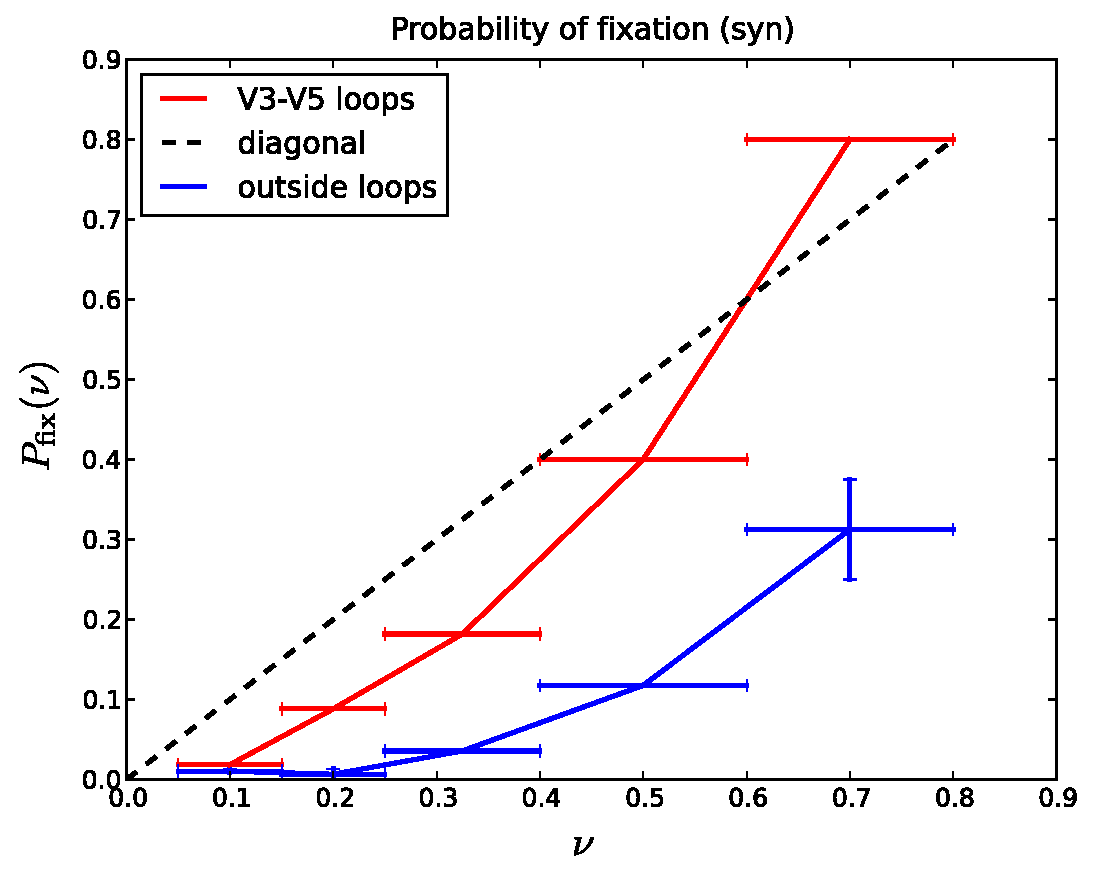
\includegraphics[width=0.49\linewidth]{Shankarappa_fixmid_syn_V_regions}}
\caption{Left panel: fixation probability of derived synonymous alleles is strongly
suppressed in C3-V5 versus other parts of the {\it env} gene, and of
nonsynonymous ones.
Right panel: especially hard is fixation of new alleles in conserved regions flanking the V
loops. The black dashed line is the prediction from neutral
theory, for comparison purposes. Data from
Refs.~\cite{shankarappa_consistent_1999, bunnik_autologous_2008}.}
\label{fig:fixp}
\end{center}
\end{figure}

The left panel of \figurename~\ref{fig:fixp} shows the fixation probability of
derived alleles seen within various frequency windows. With regard to synonymous
alleles, the average over the whole HIV genome (organce line) matches closely
the expected result from neutral theory (dashed line). A different picture
emerges when the most variable part of the genome, V1-C5 region of \env{},
is zoomed into (red line). Two independent datasets, from
refs.~\citep{shankarappa_consistent_1999, bunnik_autologous_2008} yield the same
result, i.e. that synonymous mutations hardly fix at all.

A related observation can be made on the nonsynonymous alleles (blue line).
Although we see no difference between different parts of the HIV genome, the
neutral-like shape of $P_f$ is at odds with the na\"ive expectation that most
nonsynonymous alleles reaching high frequency are to-be-fixed escape mutations.

Moreover, as illustrated in \figurename~\ref{fig:fixtimes}, the time for
synonymous alleles to reach the first boundary starting from intermediate
frequencies is of the order of 500 days which, assuming a conservative
generation time of one day~\citep{perelson_hiv-1_1996}, correspond to the same
number of generations. This time would only be possible in a neutral scenario
if the population size of HIV were extremely small, of the order of $10^3$, much
smaller then both theory and experiments
indicate~\citep{boltz_ultrasensitive_2012}.
% WE SHOULD REALLY CITE OURSELVES IN THE (HOPEFUL) FUTURE HERE :-)
\begin{figure}
\begin{center}
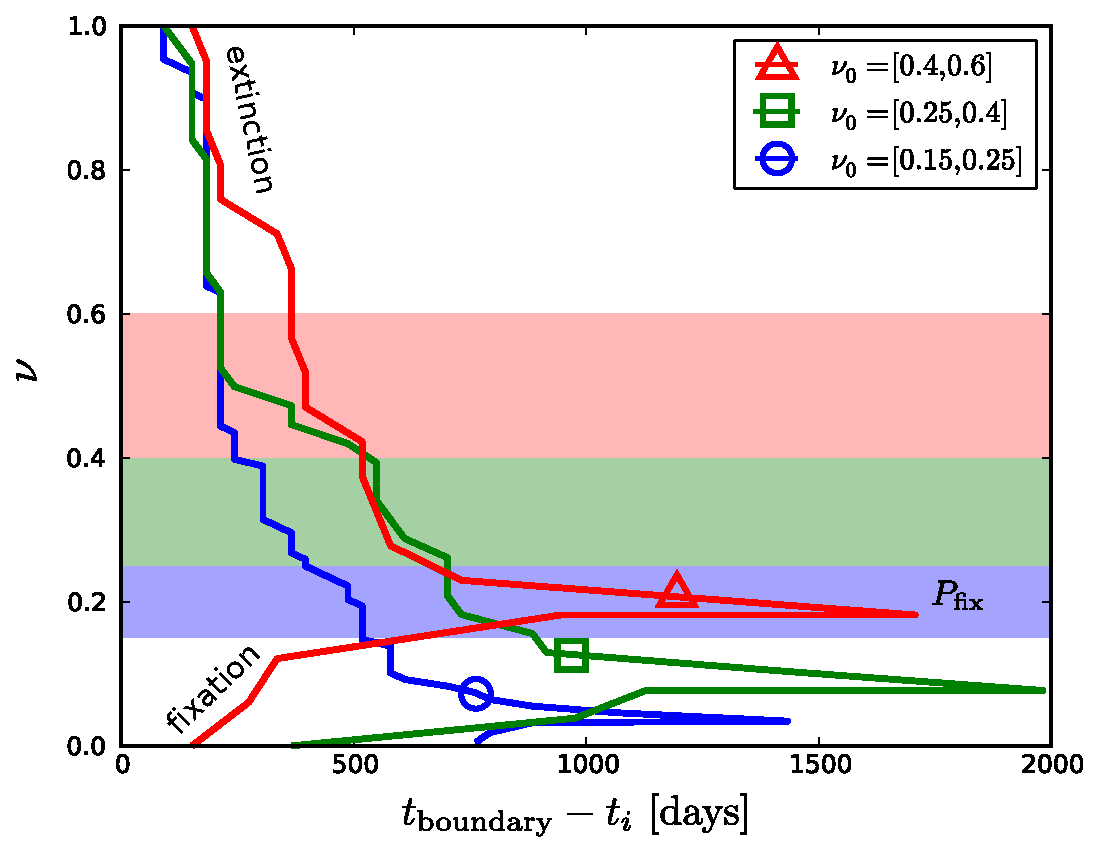
\includegraphics[width=\linewidth]{Shankarappa_fix_loss_dt_times}
\caption{Fixation or extinction times for synonymous alleles starting from
intermediate frequencies. The colored bands are the final fixation
probabilities expected from neutral theory; the observed alleles are fixed
less frequently than expected. The timescale of fixation/extinction is
approximately 500 days, corresponding to a selective effect of $\sim -0.001$.}
\label{fig:fixtimes}
\end{center}
\end{figure}

Taken together, these findings suggest that synonymous (and some nonsynonymous)
alleles are not propagating independently by genetic drift, but rather
hitchhiking on neighbouring beneficial alleles. This conclusion is also
consistent with the currently accepted estimate for the outcrossing rate of HIV,
of the order of $1\%$ per generation. Although synonymous alleles can be drafted
to high frequency by linkage and selection, they decouple on a time scale of the
order of 100 days, which is also the average time it takes a (nonsynonymous)
selected allele to spread through the population during chronic
infection~\citep{neher_recombination_2010}.

\figurename~\ref{fig:fixp} (left panel) also suggests that at least some
synonymous mutations in the V1-C5 region should be deleterious. We analyze this
hypothesis in two ways. First of all, we look for possible biological causes for
such a behaviour. Furthermore, we perform computer simulations of viral
evolution under a wide range of parameters in order to reproduce the results for
the fixation probability and study the regions of the parameter space compatible
with the observations.

One possible {\it a priori} explanation for deleterious fitness effects of
synonymous mutations is the presence of secondary structures in the viral RNA.
If any RNA secondary structures are functionally relevant for HIV replication,
mutations in nucleotides involved in those base pairs are expected to revert
more easily than by pure chance, to keep those structures in place. The
propensity of nucleotides to form base pairs in HIV has been measured
recently\citep{watts_architecture_2009}, and the HIV genome has resulted to be
highly structured~\citep{forsdyke_reciprocal_1995, watts_architecture_2009}.
Watts {\it et al.} have measured the propensity of any nucleoside to be attacked by
external chemicals (SHAPE reactivity) and shown that a higher reactivity
corresponds to a smaller likelihood of being involved in an RNA helix. As far as
the V1-C5 region is concerned, it has been shown that the short C1-5 regions
have a high tendency to form {\it insulating
stems}~\citep{watts_architecture_2009, sanjuan_interplay_2011}. Since the V1-5
loops have to be highly variable to ensure immune escape, their destabilizing
contribution to the viral RNA structure is though to be buffered by the
surrounding, base-pair rich stems. To test whether or not insulating stems might
be the reason for the reduced fixation probability, we partition the data
depending on their position in the V1-C5 region. Consistently with the
expectations, $P_f$ is more heavily readuced in the stems than in
the loops (see \figurename~\ref{fig:fixp}, right panel).

Despite this indirect result supporting the involvement of RNA secondary
structure in the deleterious effects of synonymous mutations in V1-C5, we set
out to seek more direct evidence. We partition all synonymous alleles observed
at intermediate frequencies above 10-15\% depending on their final destiny
(fixation or extinction). Subsequently, we align our sequences to the reference
NL4-3 strain used in ref.~\citep{watts_architecture_2009} and assign them SHAPE
reactivities. As shown in \figurename~\ref{fig:SHAPE} (left panel) in a
cumulative histogram, the reactivity of fixed alleles are systematically larger
than of alleles that are doomed to extinction. In other words, alleles that are
likely to be breaking RNA helices are also more likely to revert and finally be
lost from the population.
\begin{figure}
\begin{center}
\subfloat{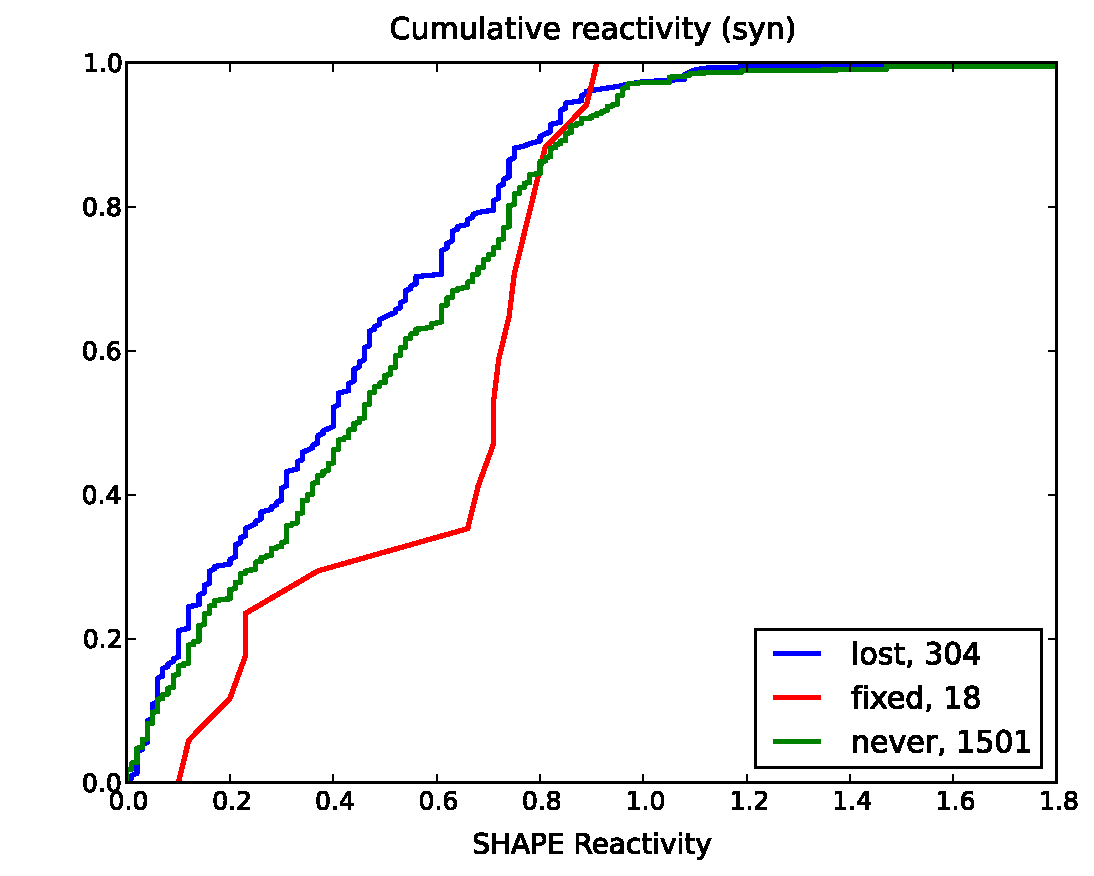
\includegraphics[width=0.49\linewidth]{mixed_Shankarappa_Bunnik2008_Liu_fixation_reactivity_Vandflanking_fromSHAPE}}
\subfloat{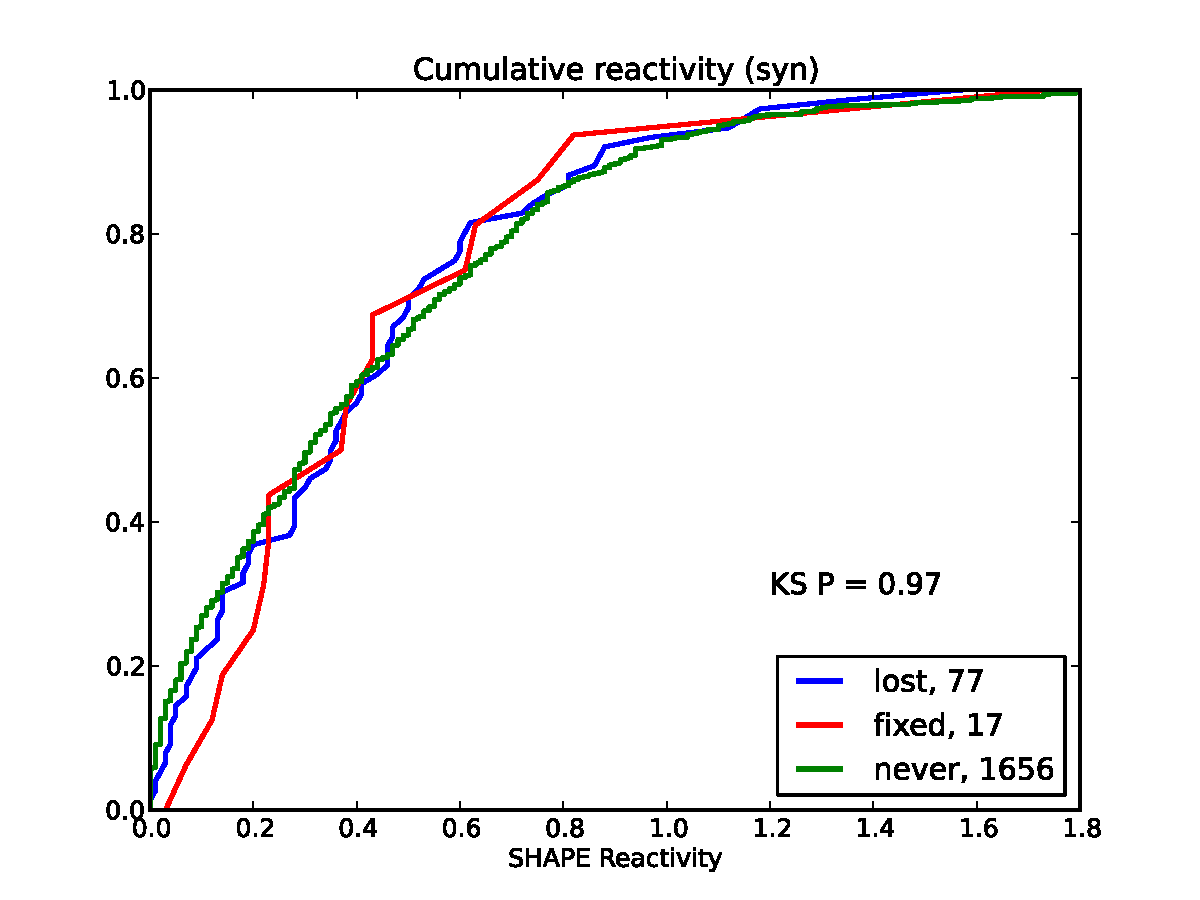
\includegraphics[width=0.49\linewidth]{mixed_Shankarappa_Bunnik2008_Liu_fixation_reactivity_nonVandflanking}}
\caption{Watts et al. have measured the reactivity of HIV nucleotides to {\it
in vitro} chemical attack and shown that some nucleotides are more likely to
be involved in RNA secondary folds. C1-C5 regions, in particular, show
conserved stem-loop structures~\citep{watts_architecture_2009}. We show that
among all derived alleles in those regions reaching frequencies of order one,
there is a negative correlation between fixation and involvement in a base
pairing in a RNA stem (left panel). The rest of the genome does not show any
correlation (right panel). There might be too few silent polymorphisms in the
first place, or the signal might be masked by non-functional RNA
structures. Data from Refs.~\cite{shankarappa_consistent_1999,
bunnik_autologous_2008, liu_selection_2006}.}
\label{fig:SHAPE}
\end{center}
\end{figure}

Since the insulating stems are not the only RNA secondary structures found by
the authors of ref.~\citep{watts_architecture_2009}, we repeated the same
partitioning based on fate on the rest of the HIV genome. As shown in the right
panel of \figurename~\ref{fig:SHAPE}, there is no evidence that a similar
mechanism is acting outside of the V1-C5 region. This is not fully surprising,
because it is well known that single stranded RNA chains tend to form a lot of
spontaneous structures, most of which have no biological function. Furthermore,
the averaging over many different genomic regions might worsen the
signal-to-noise ratio, which is already quite low, and result in
indistinguishable histograms.

In addition to RNA secondary structure, we have considered other possible
explanations for a fitness effect of synonymous mutations, in particular codon
usage bias (CUB). HIV is known to prefer A-rich codons over highly expressed
human housekeeping genes~\citep{jenkins_extent_2003}. Moreover, codon-optimized
and -pessimized viruses have recently been generated and shown to replicate
better or worse than wild type strains,
respectively~\citep{li_codon-usage-based_2012, ngumbela_quantitative_2008,
coleman_virus_2008}. We do not found, however, evidence for any contribution of
CUB to the ultimate fate of synonymous alleles. Several lines of thought support
this result. First of all, although codon-optimized HIV seems to perform better
{\it in vitro}, the distance in CUB between HIV and human genes is not shrinking
at the macroevolutionary level. Second, within a single patient, we do not
observe any bias towards more human-like CUB in the synonymous mutations that
reach fixation rather than extinction. Third, it is a common phenomenon for
retroviruses to use variously different codons from their hosts, and CUB effects
on fitness are thought to be so small that divergent nucleotide composition has
been suggested as a possible mechanism for viral
speciation~\citep{bronson_nucleotide_1994}. Fourth, CUB in the V1-C5 region is
not very different from other parts of the HIV genome, whereas the reduced
fixation probability is only observed there. In conclusion, although we cannot
exclude an effect of CUB on fitness as a general rule, we expect it to be a
minor effect in our context.

We also perform computer simulations of evolving viral population under
selection and rare recombination. For this purpose, we use the recently
published package FFPopSim, which includes a module dedicated to intrapatient
HIV evolution~\citep{zanini_ffpopsim:_2012}. We analyze many combination of
parameters such as population size, recombination rate, selection coefficient
and density of escape mutations, epitope length, deleterious effect of
synonymous mutations. The purpose of the simulations is to probe the population
genetics mechanisms required to reproduce the fixation probabilities of
\figurename~\ref{fig:fixp}, simultaneously for synonymous and nonsynonymous
alleles.

The main result of the simulations is that genetic draft can indeed generate a
depression in fixation probabilities, but only under relatively tight
circumstances. In terms of model confidence, this is a good result: the
probability of obtaining the experimental curves by pure chance is negligible.
\figurename~\ref{fig:simfixp} shows two instances of successful simulations.
\begin{figure}
\begin{center}
\subfloat{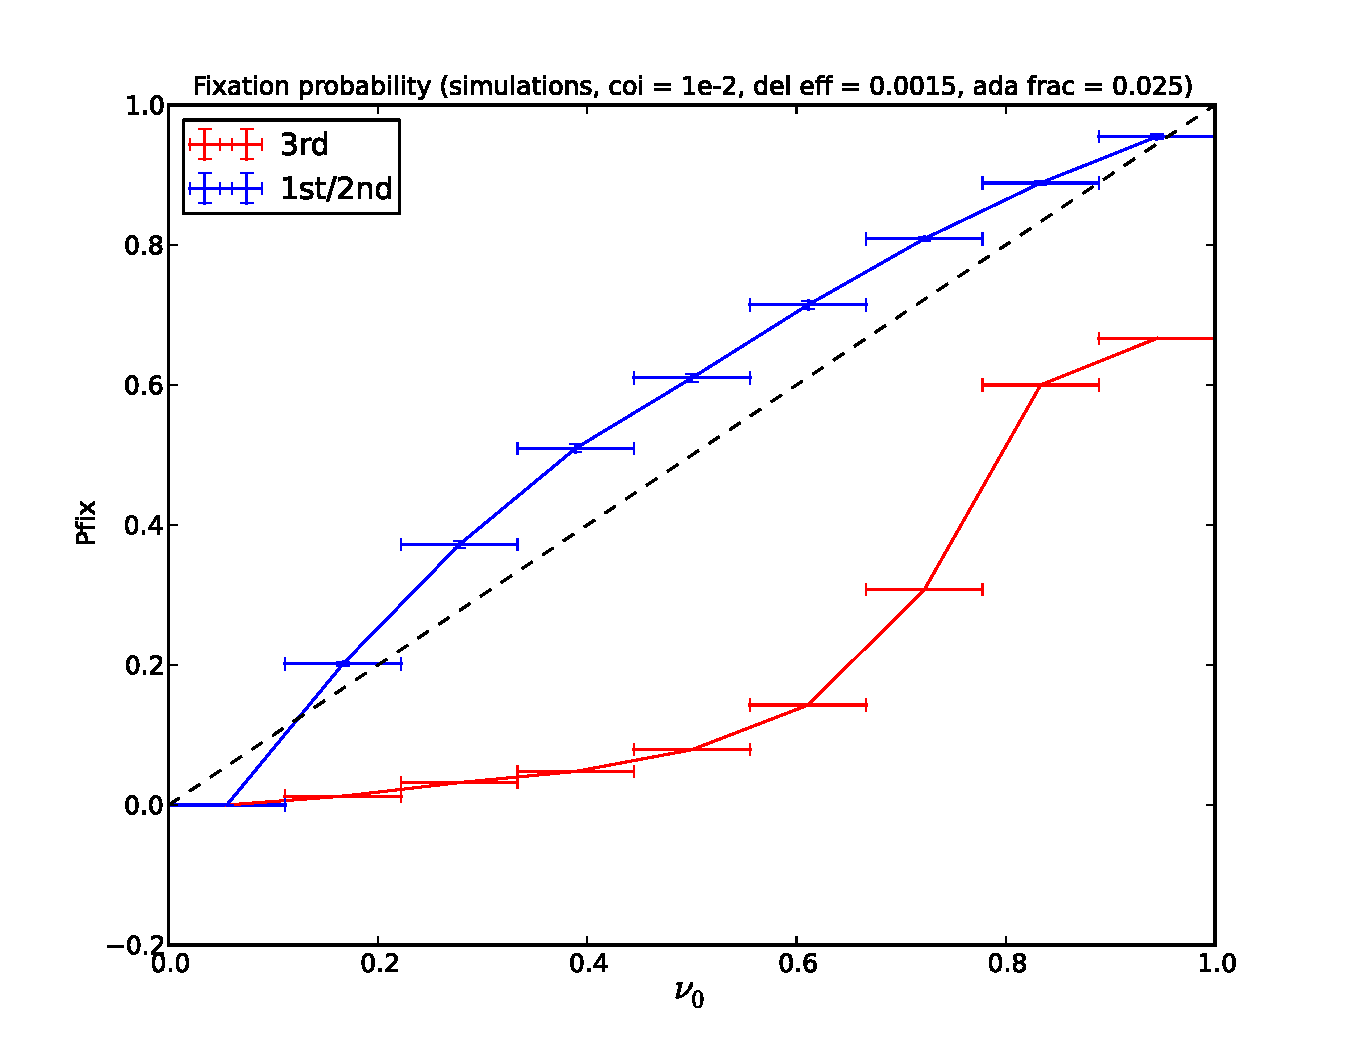
\includegraphics[width=0.49\linewidth]{fixation_probability_shortgenome_N_1e4_epitopes_example_longer}}
\subfloat{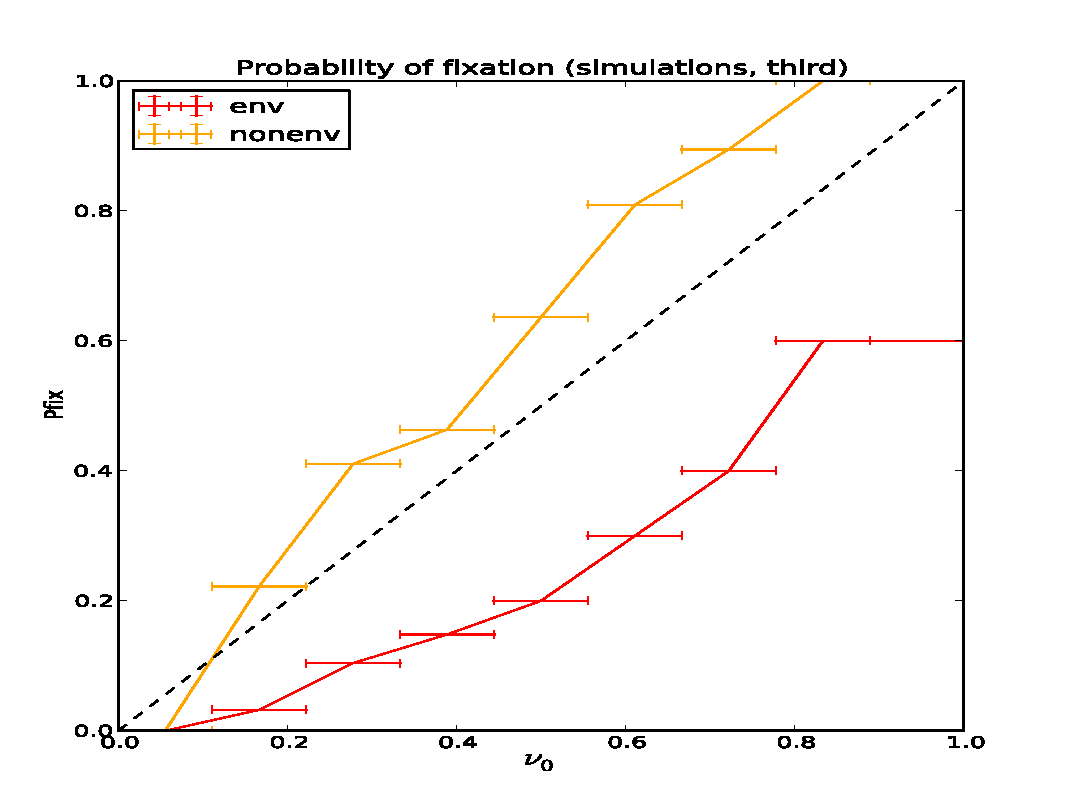
\includegraphics[width=0.49\linewidth]{fixation_probability_N_1e4_3ingredients_3rddel_envnonenv_stopall}}
\caption{Simulations show that the suppression of fixation probability can be
generated by linkage to sweeping nonsynonymous alleles nearby. Two possible
scenarios are competition between escape mutants (left panel) and time-dependent
selection due to immune sytem recognition (right panel).}
\label{fig:simfixp}
\end{center}
\end{figure}

First of all, in order for $P_f$ to be reduced to levels seen in the data, most
synonymous mutants habe to be slightly deleterious. The reason is that if
synonymous alleles are an even mixture of deleterious and neutral ones, the
latter are much more likely to be carried to high frequencies by genetic draft,
because they present no burden to escape mutations. The synonymous $P_f$ is then
dominated by these neutral alleles and the depression induced by the few
deleterious ones becomes undetectable.

Furthermore, the two crucial parameters that control the fixation probability
are the following: (a) the deleterious effects of hitchhikers compared to
the beneficial effects of escape mutants, and (b) the density of escape
mutations. Intuitively, a higher density of escape mutations (i.e., epitopes)
enables a larger degree of genetic draft, because escape mutations start to
combine and their effects add up. In \figurename~\ref{fig:simheat} (left panel),
we show that this is indeed the case in simulations. For any combination of
parameters, we get a curve like those shown in \figurename~\ref{fig:simfixp} and
we measure the area between the curve and the diagonal (neutral prediction). An
area around 0.20 to 0.35 correspond to a concave curve; an area of 0.45 means no
genetic draft at all; an area of 0 means a neutral-like fixation probability.
The data-like parameter region that produces concave $P_f$ curves is roughly
marked by the ellipse and confirms the aforementioned intuitive expectation.
\begin{figure}
\begin{center}
\subfloat{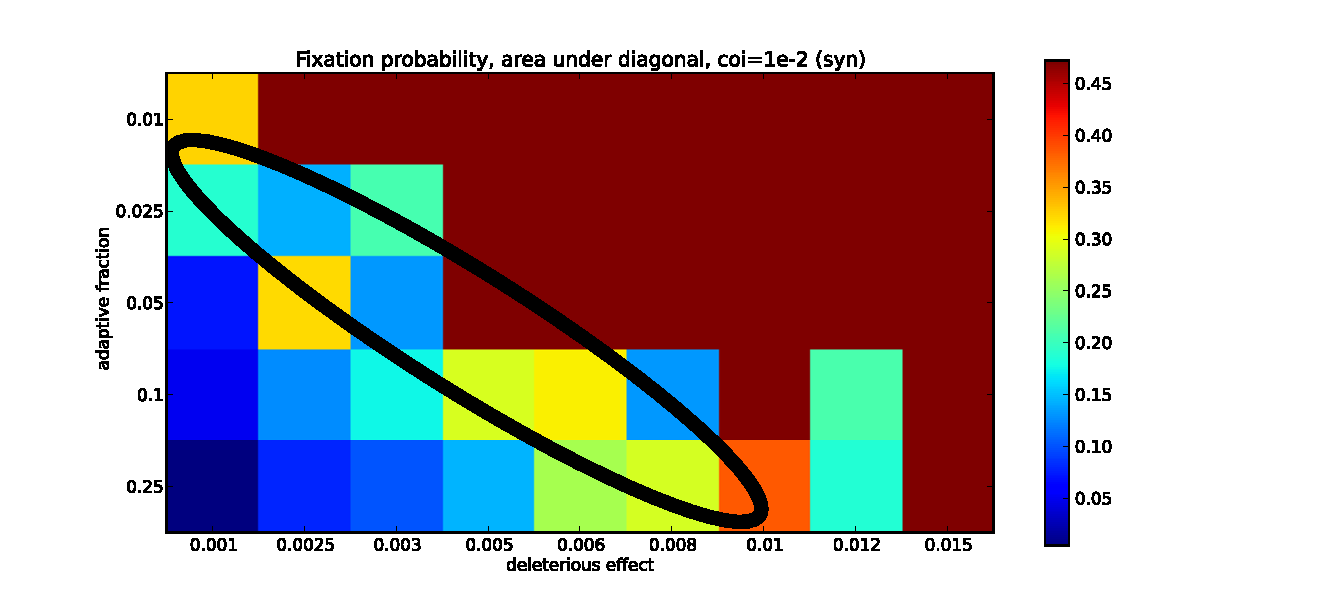
\includegraphics[width=0.49\linewidth]{fixation_loss_shortgenome_area_ada_frac_del_eff_coi_0_01_nescepi_6_heat.pdf}}
\subfloat{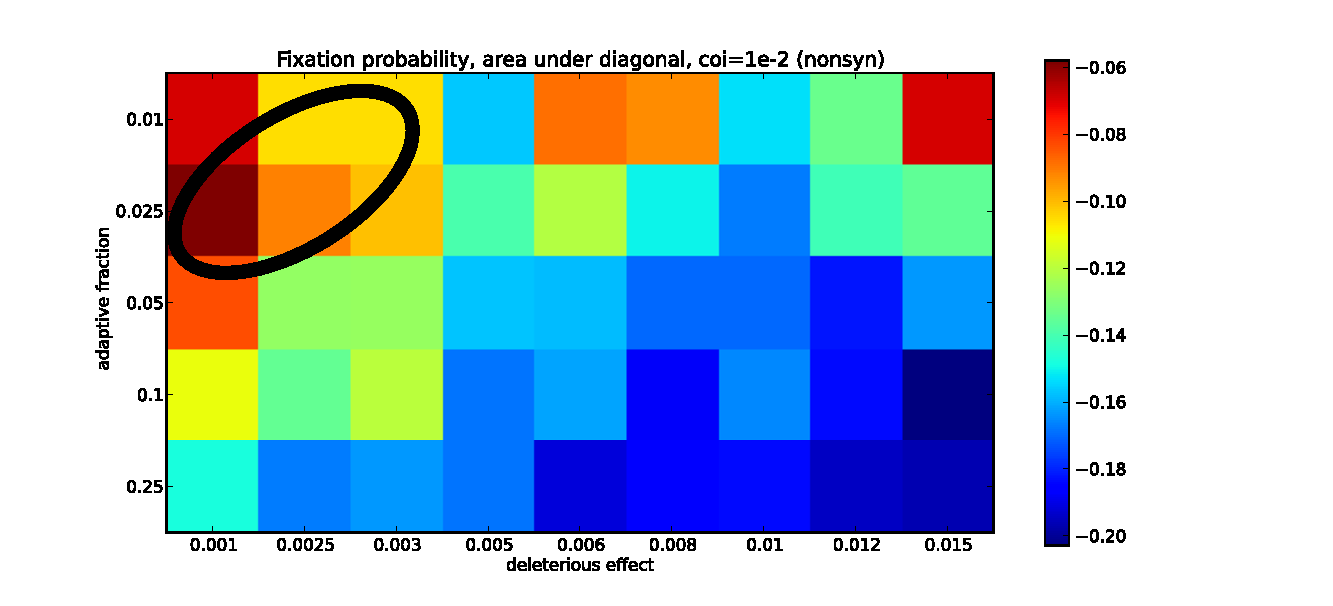
\includegraphics[width=0.49\linewidth]{fixation_loss_shortgenome_area_ada_frac_del_eff_coi_0_01_nescepi_6_nonsyn_heat.pdf}}
\caption{Simulations on the escape competition scenario show that the density of
 selective sweeps and the size of the deleterious effects of synonymous
 mutations are the main driving forces of the phenomenon. A convex fixation
 probability is recovered, as seen in the data, along the diagonal (left panel):
 more dense sweeps can support more deleterious linked mutations. The density of
 sweeps is limited, however, by the nonsynonymous fixation probability, which is
 quite close to neutrality (right panel). Moreover, strong competition between
 escape mutants is required, so that several escape mutants are ``found'' by HIV
within a few months of antibody production.}
\label{fig:simheat}
\end{center}
\end{figure}

Third, the effects of more dense escape mutations also affects the fixation
probability of {\it nonsynonymous} alleles. In real data, among all
nonsynonymous changes, there is no way to distinguish {\it a priori} between
escape mutations and hitchhikers. The fixation probability of nonsynonymous
derived alleles is an average over both, weighted by their abundances at the
starting frequency. In case of denser epitopes, this average is enriched in
escape mutations, most of which are destined to fix as soon as they reach their
establishment frequency $(sN)^{-1} \ll 0.1$~\citep{desai_beneficial_2007}. The
measured $P_f$ for nonsynonymous alleles in HIV is, however, in hardly any
excess above the neutral line (see \figurename~\ref{fig:fixp}, blue line). In
order to reconcile simulations with data on this point, several requirements
have to be met. First of all, the density of epitopes has to be fairly small,
lest they dominate the average and cause a strong rise in $P_f$. The parameter
region compatible with the data is indicated in the right panel of
\figurename~\ref{fig:simheat} with a circle in the top-left corner,
corresponding to deleterious effects of synonymous changes of roughly $-0.001$.

Moreover, even at the smallest epitope densities for which genetic draft is
still effective, it is still much more likely for an escape mutation to both
reach a high frequency and subsequently fix, compared to a nonsynonymous
hitchhiker. In HIV, however, as shown in \figurename~\ref{fig:fixtimes}, it is
quite common for a nonsynonymous mutation (solid lines) to reach majority quicky
and yet eventually get extinct. This conundrum is suggestive of an active
mechanism, in real HIV infections, for decreasing the fitness of escape mutants
over time. We test two possible such mechamisms that are biologically plausible
and find some evidence in the clinical literature: time-dependent selection and
within-epitope competition. The former concept refers to the possibility that
the host immune system slowly recognizes the escape mutants and, by deploying
its countermeasures (antibodies and killer T cells), reduces its fitness during
a selective sweep, dooming it to extinction despite the initial quick rise in
frequency. An example for the fixation probabilities generated by this kind of
models is shown in \figurename~\ref{fig:simfixp} (right panel). This scenario
finds some backing in the clinical literature: an antibody response to escape
mutants is indeed present; the delay of this response compared to appearance of
the escape mutation, a few months, matches the average sweep time of an escape
mutant. It is therefore not unlikely that the immune system catch the mutant
during the sweep and neutralize it before fixation~\citep{richman_rapid_2003,
bunnik_autologous_2008}. The alternative scenario, however, namely
within-epitope competition, is also valid. The basic idea is that, since the
mutation rate of HIV is high, several different escape mutations can be seeded
at the same time and start to spread. Their fitness benefits are not additive,
because each of them is essentially sufficient to warrant invisibility to the
host immune system (e.g. to suppress antibody binding). As a consequence, the
fastest allele to establish is most likely to reach fixation; later escape
mutants can still reach frequencies of order one because they initially only
replace wild type viruses; they are eventually swept away by the more abundant,
early established mutant. This kind of epistatic interactions within epitopes is
proven able to reduce fixation probabilities in simulations
(\figurename~\ref{fig:simfixp}, left panel). Furthermore, the emergence of
multiple sweeping nonsynonymous mutations in real HIV infections has been shown
previously~\citep{moore_limited_2009}.

\section{Discussion}
In the HIV research community, synonymous changes have been known for a long
time to have potential fitness effects, for instance via the RRE element or the
priming of RT via tRNA$^\text{Lys3}$~\citep{fernandes_hiv-1_2012,
paillart_vitro_2002}. Despite the large {\it corpus} of biochemical studies on
these phenomena, the evolutionary significance of nonneutral synonymous changes
reimains to be assessed. In this study, we show that, in the epitope-rich V1-C5
\env{} region, synonymous changes with deleterious effects are actively lost
during the course of the infection. Note that, although most of these alleles
are indeed rare at the population level, i.e. across HIV-infected subjects, that
fact alone is not sufficient to infer fitness effects, because of the
confounding effect of phylogeny. Conversely, the positive correlation between
intrapatient extinction and interpatient rarity implies, on the light of our
findings, that these alleles should be constantly depleted from the pool of
circulating HIV strains by natural selection. A mechanistic insight into this
process is not trivial, however, because the time scale of the intrapatient
depletion is long, $s^{-1} \sim 10^3~\text{days}$, whereas transmission is
thought to happen mostly during early infection~\citep{brenner_high_2007}.

With respect to the correlation with RNA seconary structure, functional
significance of the insulating stems has been proposed
previously~\citep{watts_architecture_2009, sanjuan_interplay_2011}, but its
direct microevolutionary consequences are less clear. Our analysis is akin to
that in ref.~\citep{sanjuan_interplay_2011} in terms of overall goals, but
provides direct evidence that insulating stems are relevant for viral fitness
{\it in vivo}. In absence of clear-cut biochemical experiments, our results
confirm the hypothesis that insulating stems might be needed to organize the
viral RNA during packaging in such a way as to avoid unwanted structures caused
by mutations in the hypervariable loops. In addition, although the fitness
effects involved are quite small (ten times smaller than the typical benefit of
an escape mutation), the consistency across unrelated patients makes these stems
an attractive potential target for therapeutic drugs. Unfortunately, our
approach yields a rather weak, if locally highly significant, signal. Whether or
not similar RNA secondary structures are present in other regions of the genome
remains largely an unanswered question, although we do not find evidence in this
sense. 

As far as population genetics models are concerned, our study uncovers the
subtle balance of evolutionary forces governing intrapatient HIV evolution. The
fixation and extinction times and probabilities represent a rich and simple
summary statistics to test sequencing data and computer simulation upon, as
noted independently in ref.~\citep{strelkowa_clonal_2012} in the context of
influenza. Furthermore, our results emphasize the inadequacy of independent-site
models of HIV evolution, especially in the light of transient effects on
sweeping sites, such as time-dependent selection and within-epitope negative
epistasis. Although a final word about which of these mechanisms is more
widespread is yet to be spoken, both intuition and biological evidence from the
literature support a mixed scenario~\citep{richman_rapid_2003,
moore_limited_2009}. Note also that, unlike influenza, HIV does recombine if
rarely, hence clonal interference as studied in
ref.~\citep{strelkowa_clonal_2012} is only a short-term effect. In conclusion,
we regard two consequences of this state of affairs as particularly relevant for
clinical purposes. On the one hand, the intervention of the host immune system
appears, if late, effective in fighting escape mutants, so that an active
stimulation of the host immune systems towards a more prompt response might be a
viable treatment route. On the other hand, if HIV is indeed able to generate
several escape mutants at the same time, as both data and calculations seem to
indicate, an early response against some of them might not suffice to control
the viral load.

\section{Methods}
\comment{to be written\dots}
\section*{Acknowledgements}
\comment{to be written\dots}


%%%%%%%%%%%%%%%%%%%%%%%%%%%%%%%%%%%%%%%%%%%%%%%%%%%%%%%%%%%%%%%%%%%%%%%%%
\bibliographystyle{natbib}
\bibliography{bib}
%%%%%%%%%%%%%%%%%%%%%%%%%%%%%%%%%%%%%%%%%%%%%%%%%%%%%%%%%%%%%%%%%%%%%%%%%
\end{document}
%%%%%%%%%%%%%%%%%%%%%%%%%%%%%%%%%%%%%%%%%%%%%%%%%%%%%%%%%%%%%%%%%%%%%%%%%

